\documentclass[a4paper]{article}
% Kodowanie latain 2
%\usepackage[latin2]{inputenc}
\usepackage[T1]{fontenc}
% Można też użyć UTF-8
\usepackage[utf8]{inputenc}

% Język
\usepackage[polish]{babel}
% \usepackage[english]{babel}

% Rózne przydatne paczki:
% - znaczki matematyczne
%\usepackage{amssymb}
\usepackage{amsmath, amsfonts}
% - wcięcie na początku pierwszego akapitu
\usepackage{indentfirst}
% - komenda \url 
\usepackage{hyperref}
% - dołączanie obrazków
\usepackage{graphicx}
% - szersza strona
\usepackage[nofoot,hdivide={2cm,*,2cm},vdivide={2cm,*,2cm}]{geometry}
\usepackage{lmodern}
\usepackage{changepage}
\usepackage{pythonhighlight}
\frenchspacing
\title{\emph{The Strength Pareto Evolutionary
Algorithm (SPEA)}}
\author{Piotr Piesiak}
\begin{document}
\maketitle
\section{Optymalizacja wielokryterialna - definicje}
Zajmujemy się problemem maksymalizacji / minimalizacji wielu funkcji kosztów. $$ y = f(x) = (f_1(x), f_2(x), ... ,f_n(x)) $$
Gdzie x to wektor parametrów: $$ x = (x_1, x_2, ... , x_m) $$
Problem minimalizacji n funkcji kosztów polega na tym, że nie możemy jednoznacznie stwierdzić, który wektor $y$ jest lepszy. Próbujemy zatem znaleźć zbiór rozwiązań Pareto optymalnych - należących do frontu Pareto. Mówimy, że $x_1$ dominuje $x_2$ wtw
\begin{enumerate}
\item $\forall_{i \in \{1,2,...,n\}} f_i(x_1) \leq f_i(x_2)$
\item $\exists_{i \in \{1,2,...,n\}} f_i(x_1) < f_i(x_2)$
\end{enumerate}
Rozwiązanie $x$ jest optymalne w sensie Pareto, jeśli nie istnieje żadne inne rozwiązanie, które je dominuje (jest niezdominowane). Na (rys. ~\ref{fig:f_pareto}) możemy zobaczyć front Pareto (problem minimalizacji). Punkty A,B dominują punkt C, ale nie dominują siebie nawzajem - dlatego leżą na froncie Pareto.
\begin{figure}[htbp]{}
\centerline{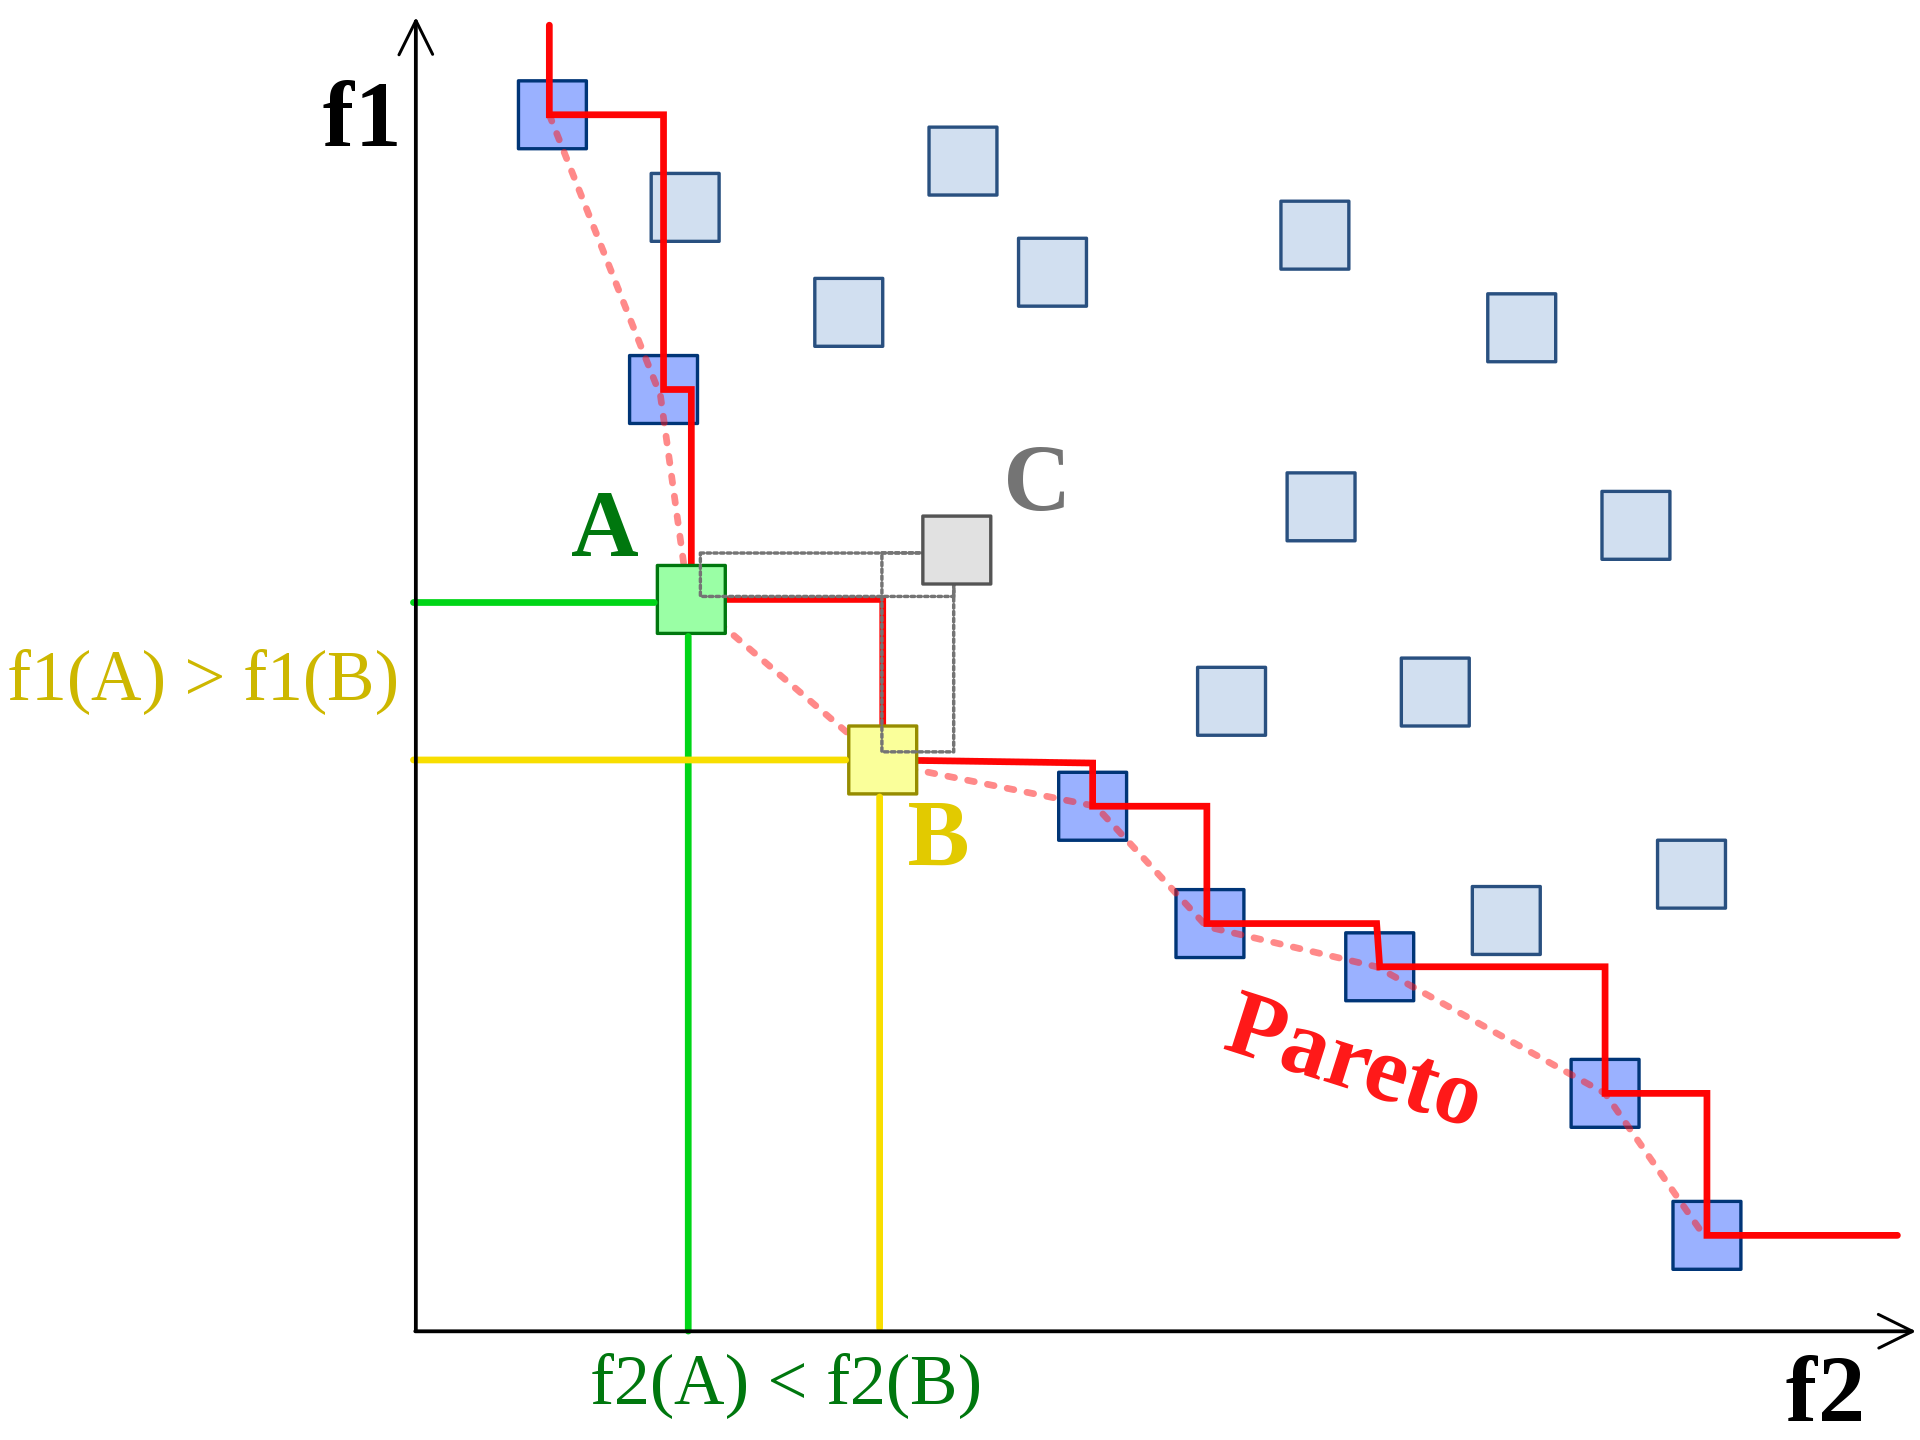
\includegraphics[scale=.13]{Front_pareto.svg.png}}
\caption{Przykład frontu Pareto (źródło: wikipedia/Multi-objective\_optimization)}
\label{fig:f_pareto}
\end{figure}
\section{Algorytm SPEA}
\subsection{Zarys algorytmu}
The Strength Pareto Evolutionary
Algorithm - algorytm zaporponowany przez Eckarta Zitzler'a i Lothara Thiel'a w 1998 roku. Jego głownymiu cechami są:
\begin{enumerate}
\item Wykorzystywanie optimum w sensie Pareto
\item Przechowywanie punktów niezdominowanych w osobnym zbiorze (obok populacji) nazywanym zbiorem Pareto
\item Redukowanie liczby osobników w zbiorze Pareto i dbanie o zachowanie charakterystyki frontu Pareto
\item Przystosowanie osobnika w populacji zależy tylko od osobników w zewnętrznym zbiorze
\item Selekcje, Krzyżowanie i Mutacje wykonujemy na sumie zewnetrznego zbioru i populacji
\end{enumerate}

\begin{figure}[htbp]{}
\centerline{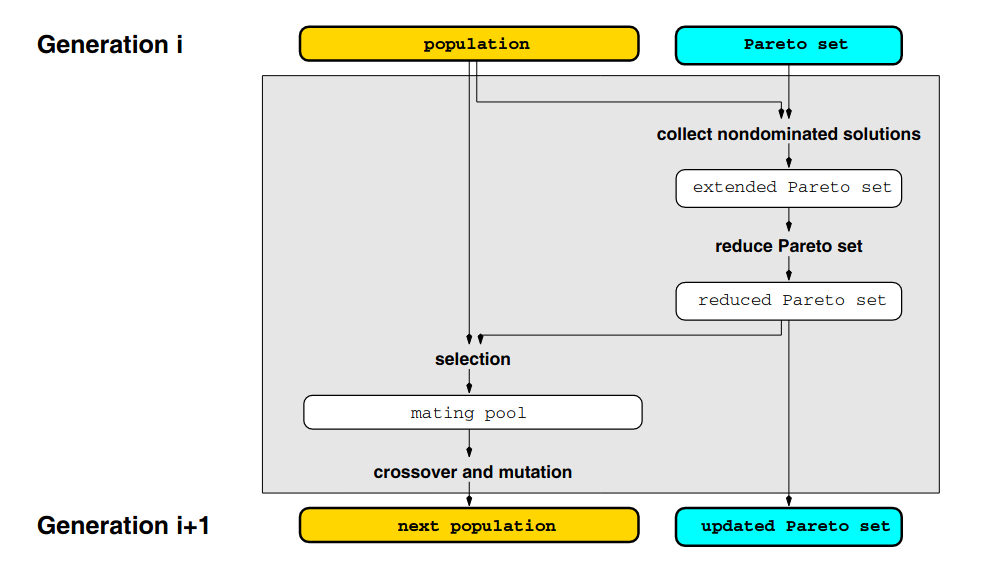
\includegraphics[scale=.45]{szkic_alg.png}}
\caption{Szkic SPEA (źródło: praca Zitzlera i Thiela, 1998)}
\label{fig:szkic_alg}
\end{figure}

\subsection{Selekcja}
Każdemu osobnikowi ze zbioru Pareto przypisujemy jego siłę $s \in [0,1]$, parametr ten jest proporcjonalny do ilości zdominowanych osobników. Siła $S(i)$ osobnika $i$ wyliczana jest następująco: $$S(i) = \frac{n}{N + 1}$$gdzie $n$ to liczba osobników w populacji zdominowanych przez osobnika $i$, a $N$ to liczność populacji. Wartością przystosowania osobnika ze zbioru Pareto jest jego siła.
Na tej podstawie osobniki populacji (czyli osobnego zbioru) są rankingowane względem zbioru Pareto $P$ w sposób : $$F(i) =  \sum_{j \succeq  i, j \in P}S(j) + 1$$
Czyli wartością przystosowania osobnika $i$ jest powiększona o jeden suma sił osobników ze zbioru Pareto, które dominują $i$. Dodanie jedynki zapewnia, że ranking osobników ze zbioru Pareto będzie zawsze lepszy od rankingu osobnika z populacji. Przydaje się to w sytuacji, gdy osobnika $i$ dominuje tylko jeden osobnik $j$. Przez lepszego osobnika rozumiemy osobnika o mniejszej wartości przystosowania.
\newpage
\begin{figure}[htbp]{}
\centerline{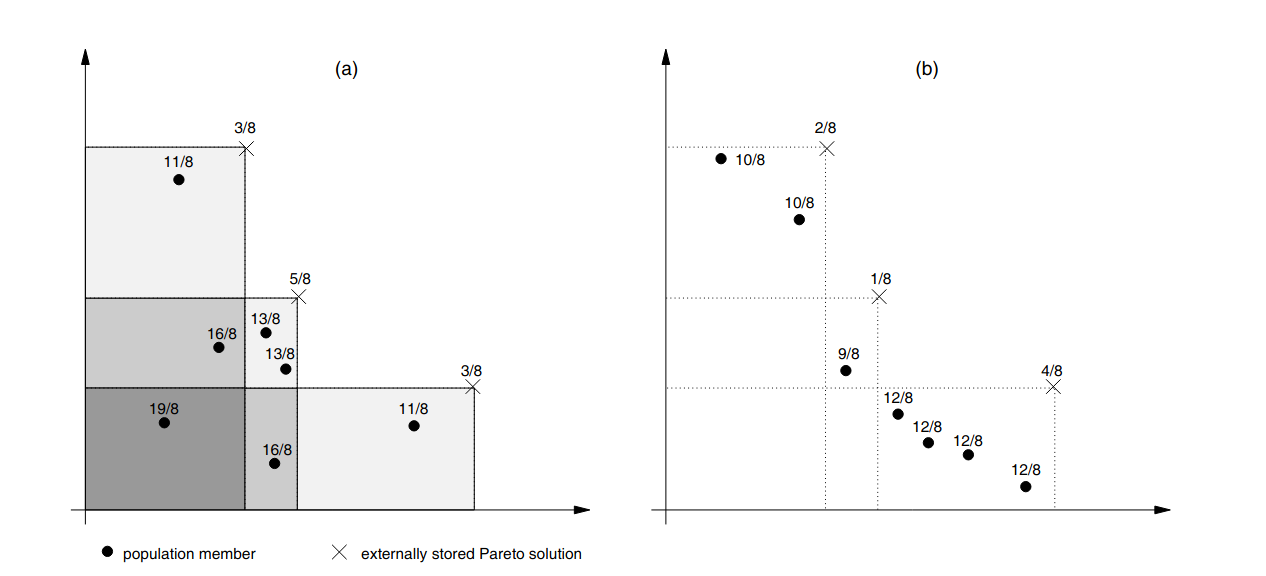
\includegraphics[scale=.35]{strength.png}}
\caption{Wartości przysotosowania poszczególnych osobników - problem maksymalizacji (źródło: praca Zitzlera i Thiela, 1998)}
\label{fig:sila}
\end{figure}
Na rysunku widać dwa różne scenariusze - po lewej wartość przystosowania zależy od ilości dominujących punktów ze zbioru Pareto (zbalansowana populacja). Po prawej każdego osobnika z populacji dominuje tylko jeden punkt ze zbioru Pareto - tutaj wartość przystosowania zależy od siły osobnika z zewnetrznęgo zbioru (niezbalansowana populacja). Dzięki temu odosobnione osobniki są bardziej cenione w selekcji i nasz algorytm porusza się bardziej równomiernie.
Mając sposób na ocenienie osobników możemy przystąpić do selekcji. Autorzy zaproponowali selekcję poprzez metodę turnieju binarnego. Losujemy dwóch osobników $i,j$ z sumy populacji i zbioru Pareto. Oceniamy ich wg. wartości przystosowania $i$. Do zbioru rodziców $R$ przepuszczamy jednostkę o mniejszej wartości. Powtarzamy turniej (losowanie ze zwracaniem) aż uzyskamy odpowiednią liczbę rodziców. 
\subsection{Krzyżowanie i mutacje}
Mając już wybrany zbiór rodziców $R$, który może zawierać osobników z populacji i zbioru Pareto, możemy przystąpić do krzyżowania i mutacji. Możemy tu dostosowywać te metody w zależności od problemu. 
\subsection{Redukcja zbioru Pareto}
Musimy dbać o mały rozmiar i równomierne rozłożenie punktów w zbiorze Pareto z kilku powodów:
\begin{enumerate}
\item Nie potrzeba nam tylu punktów - dla osoby podejmującej decyzje nie jest potrzebna ogromna liczba punktów z Frontu Pareto
\item Oszczędzamy pamieć - nie uda się przechować ciągłego frontu Pareto
\item Gdy zbiór Pareto nie jest równomiernie rozłożony, poszukiwania mogą być nakierowane na tylko niektóre rejony, przez co generujemy nierównomierną populacje
\end{enumerate}
Proces redukcji zbioru Pareto ma na celu nie tylko zmniejszenie liczby osobników, ale także zachowanie charakterystyki przebiegu frontu. Algorytm redukcji dzieli podobnych osobników w $q$ grup (niech $q$ to maksymalna moc zbioru Pareto). Następnie dla każdej grupy wybierany jest osobnik reprezentujący, który zastępuje swoją grupę. Dzięki temu w zrównoważony sposób redukujemy moc zbioru Pareto do $q$.
\begin{figure}[htbp]{}
\centerline{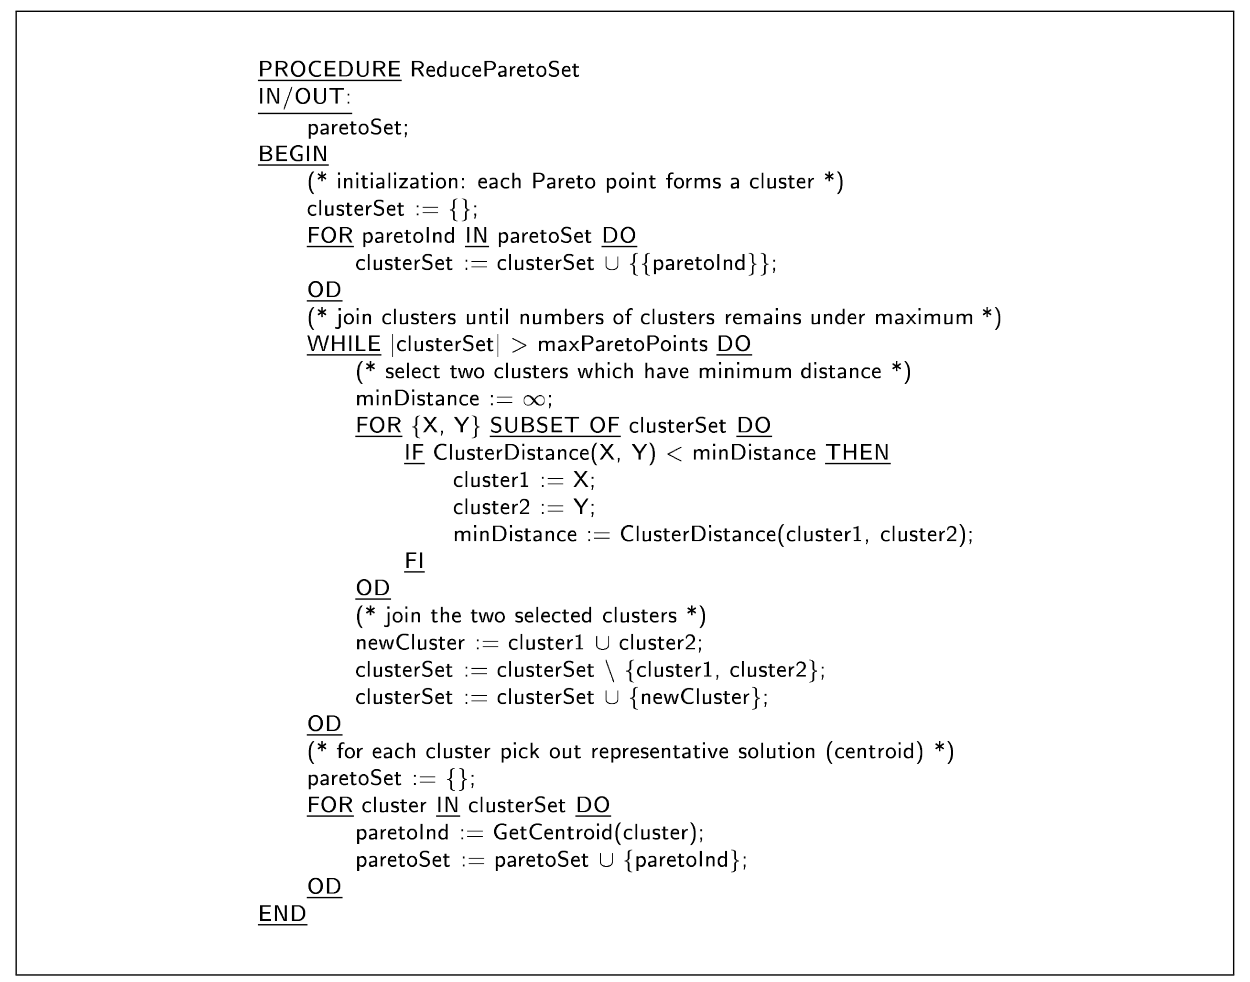
\includegraphics[scale=.25]{clustering.png}}
\caption{Pseudokod procedury podziału na grupy (źródło: praca Zitzlera i Thiela, 1998)}
\label{fig:clustering}
\end{figure}
\begin{enumerate}
\item Formowanie grup - początkowo każdy osobnik zbioru Pareto tworzy osobną grupę. W kolejnych krokach wybieramy najbliższe grupy i łączymy je w jedną. Powtarzamy tę czynność aż liczba grup zmniejszy się do wymaganej wartości.
\item  Najbliższe grupy - odległość grup $X$, $Y$ definiujemy jako średnią z odległości pomiędzy parami punktów z $X$ , $Y$, tzn. dla każdej pary punktów z $X,Y$ znajdujemy jej odległość euklideoswą i wyciągamy średnią.
\item Reprezentanci grup - mając odpowiednią ilość grup wybieramy reprezentantów. Reprezentatem grupy nazywamy centroid grupy, czyli punkt który ma najmniejszą średnią odległość do wszystkich innych punktów danej grupy. 
\end{enumerate}
\section{Działanie w praktyce - $f_2$ funkcja Shaffer'a}
Shaffer zaproponował prostą funkcję testową: 
$$f_2(x) = (g(x), h(x)) \ , g(x) = x^2, h(x) = (x-2)^2$$
Celem jest zminimalizowanie obydwu funkcji na raz. Na rys.~\ref{fig:shaffer} możemy zobaczyć wykresy dwóch funkcji i naszkicowany front Pareto. Jak łatwo sprawdzić, punkty $x$ frontu Pareto należą do przedziału $[0,2]$ - poza tym przedziałem $g$ i $h$ rośnie, zatem punkty $x \notin [0,2]$ są zdominowane.
\begin{figure}[htbp]{}
\centerline{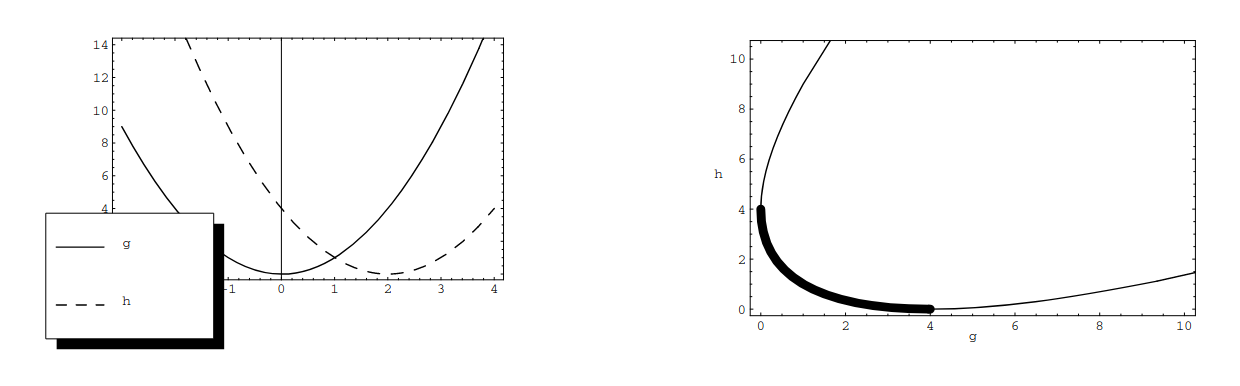
\includegraphics[scale=.35]{schaffers.png}}
\caption{Funkcja Shaffer'a i funkcja parametryczna z zaznaczonym frontem Pareto (źródło: praca Zitzlera i Thiela, 1998)}
\label{fig:shaffer}
\end{figure}

W swojej pracy Zitzler i Thiel przeprowadzili prosty test porównujący algorytm SPEA oraz VEGA (Vector Evaluated Genetic Algorithm). Algorytm VEGA polega na podziale populacji na $k$ grup, gdzie $k$ to liczba funkcji celu. Selekcja wewnątrz każdej grupy przeprowadzana jest niezależnie, względem wybranego kryterium. Mutacje i krzyżowanie są wykonywane na całej populacji. Jest to prosty algorytm optymalizujący problemy wielokryterialne. Jego podstawową wadą jest pomijanie rozwiązań pośrednich - zwracane rozwiązania maksymalizują / minimalizują zwykle jedną z funkcji celu. \\
Aby porównać efektywność algorytmu SPEA i VEGA, autorzy ustawili następujące parametry w SPEA:
\newpage
\begin{enumerate}
\item Rozmiar populacji: 95/70/30
\item Rozmiar zewnętrznego zbioru Pareto: 5/30/70
\item Prawdopodobieństwo krzyżowania: 1.0
\item Prawdopodobieństwo mutacji: 0.0
\item Liczba iteracji: 100
\end{enumerate}
Zastosowali 3 rózne kombinacje, w każdej z nich suma zbioru Pareto i populacji sumowała się do 100. Prawdopodobieństwo mutacji zostało ustawione na 0.0, aby móc porównać efektywność samego SPEA. W algorytmie VEGA użyto populacji o wielkości 100 i takich samych pozostałych parametrów. Na rys.~\ref{fig:performance} możemy zobaczyć, że algorytm SPEA poradził sobie ze znalezieniem frontu i zwrócił bardzo zrównoważone rozwiązania. W algorytmie VEGA, pomimo takiej samej sumarycznej liczby osobników, rozwiązanie jest gorsze i mniej zrównoważone.
\begin{figure}[htbp]{}
\centerline{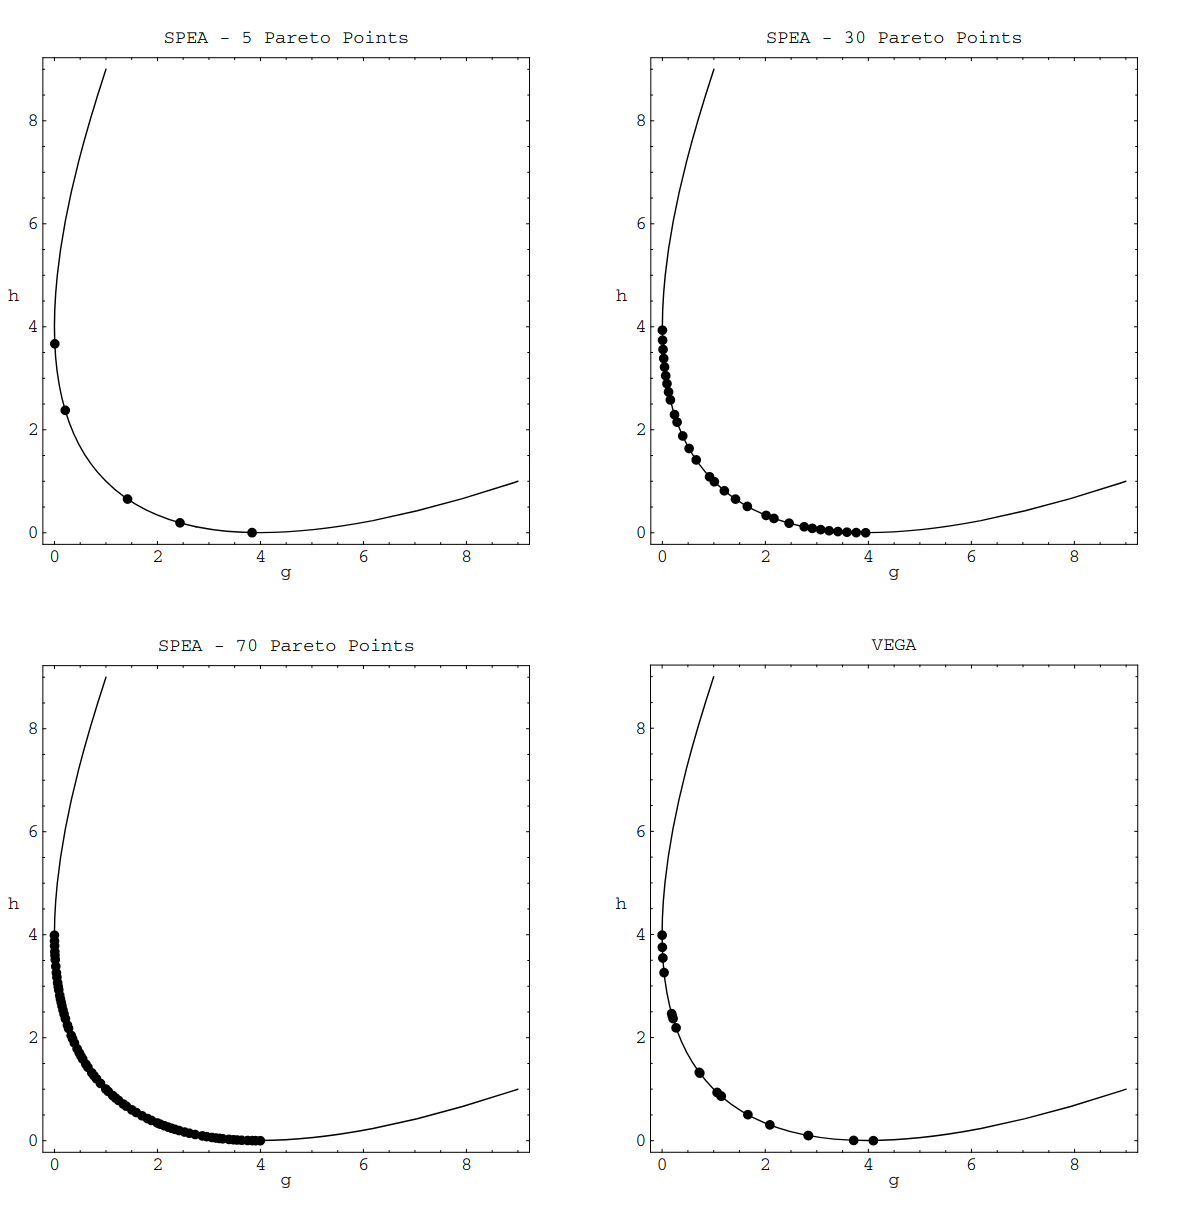
\includegraphics[scale=.30]{performance.png}}
\caption{Wyniki SPEA w porównaniu do VEGA (źródło: praca Zitzlera i Thiela, 1998)}
\label{fig:performance}
\end{figure}
\begin{thebibliography}{9}
\bibitem{texbook}
Eckart Zitzler and Lothar Thiele (1998) \href{https://sop.tik.ee.ethz.ch/publicationListFiles/zt1998a.pdf}{An Evolutionary Algorithm for
Multiobjective Optimization: The Strength Pareto Approach}.
\bibitem{texbook}
Rahman Gharari, Navid Poursalehi, Mohammadreza Abbasi, Mahdi Aghaie (2016) \href{https://reader.elsevier.com/reader/sd/pii/S1738573316300493?token=C05246879BE6CF68BC0862DBF5EC6B3BA49BC955850FBB6B93FF1D5A0D475BFF7A74823972A48F62520CAA1D1A185FE5&originRegion=eu-west-1&originCreation=20211202160112}{Implementation of Strength Pareto EvolutionaryAlgorithm II in the Multiobjective Burnable PoisonPlacement Optimization of KWU Pressurized WaterReactor}.
\bibitem{texbook}
Marcin Wściubiak (2000) \href{https://www.ii.pwr.edu.pl/~kwasnicka/tekstystudenckie/ewoptymwielokryt.pdf}{Ewolucyjna optymalizacja wielokryterialna}.
\end{thebibliography}
\end{document}